\documentclass[12pt, cn]{elegantart}

\title{数学之美 --- The Beauty of Mathematics}
\subtitle{$\me^x=\sum_{n=0}^{\infty}\frac{x^n}{n!}=1+x+\frac{x^2}{2!}+\frac{x^3}{3!}+\frac{x^4}{4!}+\frac{x^5}{5!}+\cdots$}

\author{任\ 涛}
\email{me@tomben.me}
\date{\today}
\version{3.14}

\extrainfo{This \href{https://tomben.me/the-beauty-of-mathematics/the-beauty-of-mathematics.pdf}{booklet} was proudly made with \href{https://www.latex-project.org}{\LaTeX{}} and inspired by \href{https://github.com/ElegantLaTeX/ElegantBook}{ElegantBook}. The Chinese text is set in \href{https://source.typekit.com/source-han-serif/}{Source Han Serif}\!(思源宋体)\!\! and \href{https://docs.microsoft.com/en-us/typography/font-list/kaiti}{KaiTi}\!(\textit{楷体})\!\!. The western text is set in \href{https://www.ctan.org/pkg/newtx}{newtxtext}. And the math text is set in \href{https://www.ctan.org/pkg/newtx}{newtxmath} with a few \href{https://tex.stackexchange.com/questions/200910/replace-a-few-math-symbols-in-the-newtxmath-font}{modif{}ications}. All tools mentioned are \href{https://en.wikipedia.org/wiki/Open_source}{open source}.}

\logo{logo.pdf}
\cover{cover.jpg}


\begin{document}

\maketitle

\begin{introduction}
\item 8 月底,姜勤耘同学问了我一道关于自然数前 $n$ 项和的公式。
\item 数学是晦涩难懂的,但又是美丽动人的。就像青春期的少年,当你不了解他时,觉得他是那么淘气不听话,心思一点也猜不透,可当你真正了解了他时,就会觉得他是那么美丽,那么可爱,令人感慨数学真是上帝的杰作!
\item 本文选取一些看上去非常优美的数学公式(以无穷级数为主),并加以证明,共同来领略数学的美妙。此外,本文源代码及相关附件托管在 \href{https://github.com/TomBener/the-beauty-of-mathematics}{GitHub} 上,将持续进行更新,可在 GitHub 下载最新版本。
\end{introduction}

\begin{center}
	\Large\bfseries\color{structurecolor} 目\hspace{0.5em}录 \\[5pt]
	\base{structurecolor}{87}
\end{center}
\vspace{-0.8cm}
\tableofcontents

\section{$\me$ 和 $\pi$}

\noindent 法国数学家弗朗索瓦·勒·利奧奈(Fran{\c{c}}ois Le Lionnais)\cite{le2004}曾说:
\vspace{5pt}

\begin{tcolorbox}[saying]
   Who has not been amazed to learn that the function $y = \me^x$, like a phoenix rising from its own ashes, is its own derivative? \vspace{5pt}

   有谁不被 $y = \me^x$ 惊艳过?就像浴火重生的凤凰一般,它从自身的导数中一飞冲天。
\end{tcolorbox}

\begin{figure}[h]
\centering
  \begin{tikzpicture}
  \node [below left] at (0,0) {$O$};
  \draw[->] (-4.2,0) -- (4.2,0) node[right] {$x$};
  \draw[->] (0,-0.5) -- (0,7.2) node[above] {$y$};
  \draw[color=blue, smooth, thick, domain=-4:2] plot (\x,{exp(\x)}) node[right] {$y = \me^x$};
  \end{tikzpicture}
\caption{$y = \me^x$ 一飞冲天}
\end{figure}

\begin{figure}[H]
\centering
  \begin{tikzpicture}
  \node [below right] at (0,0) {$O$};
  \draw[->] (-4.2,0) -- (7.2,0) node[right] {$x$};
  \draw[->] (0,-5) -- (0,7.2) node[above] {$y$};
  %\draw[color=red, smooth, thick, domain=-4:0.9] plot (\x,{2.5*exp(\x)});
  %\draw[color=green, smooth, thick, domain=-4:1.2] plot (\x,{2*exp(\x)});
  %\draw[color=cyan, smooth, thick, domain=-4:1.55] plot (\x,{1.5*exp(\x)});
  \draw[color=blue, smooth, thick, domain=-4:2] plot (\x,{exp(\x)}) node[above] {$y = \me^x$};
  %\draw[color=magenta, smooth, thick, domain=-4:2.6] plot (\x,{0.5*exp(\x)});
  %\draw[color=yellow, smooth, thick, domain=-4:3] plot (\x,{0.3*exp(\x)});
  %\draw[color=purple, smooth, thick, domain=-4:3.3] plot (\x,{0.2*exp(\x)});
  %\draw[color=teal, smooth, thick, domain=-4:3.7] plot (\x,{0.12*exp(\x)});
  %\draw[color=pink, smooth, thick, domain=-4:4] plot (\x,{0.08*exp(\x)});
  %
  \draw[smooth, thick, domain=-3:6.8] plot (\x,{\x}) node[right] {$y=x$};
  %
  \draw[color=red, smooth, thick, domain=0.01:1.001] plot (\x,{ln(\x)});
  \draw[color=red, smooth, thick, domain=1:7] plot (\x,{ln(\x)}) node[right] {$y = \ln x$};
  %\draw[color=purple, smooth, thick, domain=0.1:4] plot (\x,{2*ln(\x)});
  %\draw[color=teal, smooth, thick, domain=0.01:4] plot (\x,{0.5*ln(\x)});
  %\draw[color=olive, smooth, thick, domain=0.01:4] plot (\x,{0.8*ln(\x)});
  %\draw[color=brown, smooth, thick, domain=0.01:4] plot (\x,{0.5*ln(\x)});
  %\draw[color=lime, smooth, thick, domain=0.18:4] plot (\x,{2.5*ln(\x)});

  \end{tikzpicture}
\caption{指数函数与对数函数互为反函数,图像关于直线 $y=x$ 对称}
\end{figure}

此处不禁想起老何的两首打油诗:
\begin{proposition}{指数函数}{fki}
\centering
	一刀冲天刀未残,接近横轴趋无限。

	朵朵菊花集一束,愿留芬芳在人间。
\end{proposition}

\begin{proposition}{对数函数}{hyo}
\centering
	千条万条集一束,左右延伸趋无限。

	菊花旋转九十度,指对互为反函数。
\end{proposition}

在社交媒体中,每年圆周率日\footnote{圆周率日(Pi Day)是庆祝圆周率 $\pi$ 的特别日子,日期是 3 月 14 日,由圆周率最常用的近似值 3.14 而来。美国麻省理工学院首先倡议将 3 月 14 日定为国家圆周率日(National Pi Day)。2009 年美国众议院正式将每年的 3 月 14 号设定为“圆周率日”(Pi day)。3 月 14 日也是阿尔伯特·爱因斯坦的生日,卡尔·马克思和史蒂芬·霍金的忌日以及白色情人节。}之际,人们总会分享关于 $\pi$ 的名言,其中 Lisa Hoffman(丽莎·霍夫曼)的这句:
\vspace{5pt}

\begin{tcolorbox}[saying]
Love is like pi --- natural, irrational, and very important.
\vspace{5pt}

爱情就像 $\pi$ 一样 --- 自然、无理\footnote{众所周知,$\pi$ 是一个无理数。},却至关重要。
\end{tcolorbox}

可能是在丽莎·霍夫曼这句话的基础上,另外一句关于 $\pi$ 类似的话也在网络上广为流传,并且被印在 \href{https://teespring.com/shop/love-pi-math}{T-shirt} 上进行出售。
\vspace{5pt}

\begin{tcolorbox}[saying]
Love is like pi - irrational and never-ending.
\vspace{5pt}

爱情就像 $\pi$ 一样 --- 无理并且无穷无尽。
\end{tcolorbox}

$\pi$ 有多“无理”呢?下面是 $\pi$ 的 walk.\footnote{不够直观?前往{\href{https://nbremer.github.io/freshdatashapes/\#/pi-walk}{这里}}查看 $\pi$ 的动态小数位数。}

\begin{figure}[h]
	\centering
	\includegraphics[width=12cm]{pi-walk.jpg}
	\caption{100000 位小数的 $\pi$}
\end{figure}

\begin{center}
	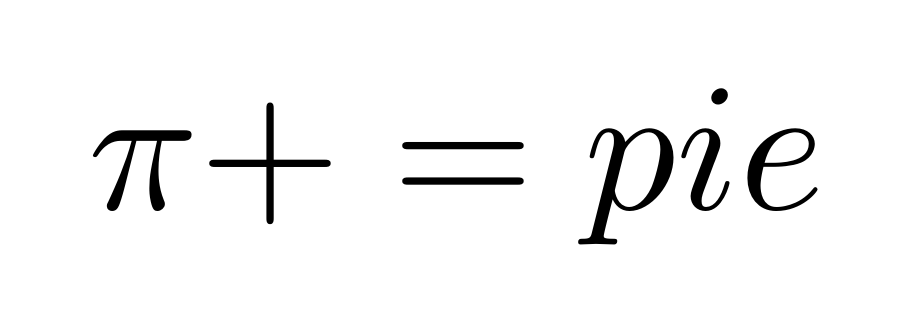
\begin{tikzpicture}
      \marmot[pie,whiskers,teeth,shadow]
      \node[anchor=east,scale=6.6,transform shape] at (-0.5,1) {$\pi + \me =\text{pie}$};
    \end{tikzpicture}
\end{center}
%\vspace{10pt}


\section{自然数幂和公式}

\begin{theorem}{自然数平方和}{qwe}
\begin{equation}
   \sum_{i=1}^{n} i^{2}=1^2+2^2+3^2+\cdots+n^2=\frac{n(n+1)(2 n+1)}{6}
\end{equation}  
\end{theorem}

\begin{definition}{自然数平方和}{oiy}
\ding{172} 方法一:利用立方差公式累加求和

观察下面的等式:
$$\begin{array}{l}
{(n+1)^{3}-n^{3}=3 n^{2}+3 n+1}, \\ {(n)^{3}-(n-1)^{3}=3(n-1)^{2}+3(n-1)+1}, \\ {\cdots \cdots} \\ {3^{3}-2^{3}=3 \cdot 2^{2}+3 \cdot 2+1}, \\ {2^{3}-1^{3}=3 \cdot 1^{2}+3 \cdot 1+1}
\end{array}$$

将以上 $n$ 个等式相加,左边消去中间项,右边提取公因式合并,得到:
$$
(n+1)^{3}-1^{3}=3\left(1^{2}+2^{2}+\dots+n^{2}\right)+3(1+2+\dots+n)+n
$$

化简整理得到:
$$
1^{2}+2^{2}+\dots+n^{2}=\frac{n(n+1)(2 n+1)}{6}
$$

\hdashrule{\linewidth}{0.5pt}{3pt}

\ding{173} 方法二:一元函数积分法

构造二次函数:
$$f(x)=x^2,\ x \in[1, n+1]$$

将区间 $[1, n+1]$ 分割为 $n$ 个区间,则每个小曲边三角形的面积为:

$$
\int_{k}^{k+1}\left(x^{2}-k^{2}\right) \md x=\left.\frac{1}{3} x^{3}\right|_{k} ^{k+1}-\left.k^{2} x\right|_{k} ^{k+1}=k+\frac{1}{3}
$$

所以曲边三角形的面积为:
\begin{align*}
   \sum_{k=1}^{n} k^{2}&=\int_{1}^{n+1} x^{2} \md x-\sum_{k=1}^{n}\left(k+\frac{1}{3}\right)\\
   &=\left.\frac{1}{3} x^{3}\right|_{1} ^{n+1}-\sum_{k=1}^{n}\left(k+\frac{1}{3}\right)\\
   &=\frac{1}{3}(n+1)^{3}-\frac{1}{3}-\sum_{k=1}^{n} k-\sum_{k=1}^{n} \frac{1}{3}\\
   &=\frac{n(n+1)(2 n+1)}{6}
   \end{align*}
\end{definition}


\begin{theorem}{自然数立方和}{ert}
\begin{equation}
     \sum_{i=1}^{n} i^{3}=1^3+2^3+3^3+\cdots+n^3=\left(\frac{n(n+1)}{2}\right)^{2}
\end{equation}
\end{theorem}

\begin{definition}{自然数立方和}{ihj}
	观察下面的等式:
$$\begin{array}{l}
{(n+1)^{4}-n^{4}=4 n^{3}+6 n^{2}+4 n+1}, \\ {n^{4}-(n-1)^{4}=4(n-1)^{3}+6(n-1)^{2}+4(n-1)+1}, \\ {\cdots \cdots} \\ {3^{4}-2^{4}=4 \cdot 2^{3}+6 \cdot 2^{2}+4 \cdot 2+1}, \\ {2^{4}-1^{4}=4 \cdot 1^{3}+6 \cdot 1^{2}+4 \cdot 1+1}
\end{array}$$

将以上 $n$ 个等式相加,左边消去中间项,右边提取公因式合并,得到:
$$
(n+1)^{4}-1^{4}=4\left(1^{3}+2^{3}+\dots+n^{3}\right)+6\left(1^{2}+2^{2}+\dots+n^{2}\right)+4(1+2+\dots+n)+n$$

化简整理得到:
$$
1^{3}+2^{3}+\dots+n^{3}=\left(\frac{n(n+1)}{2}\right)^{2}$$
\end{definition}

\noindent 自然数 $n$ 次幂和公式的规律如下:
$$
\begin{array}{l}
{\sum_{i=1}^{n-1} i=\frac{1}{2} n^{2}-\frac{1}{2} n}\,, \quad\quad\quad\quad\quad\;\ {\sum_{i=1}^{n-1} i^{2}=\frac{1}{3} n^{3}-\frac{1}{2} n^{2}+\frac{1}{6} n} \\[15pt] {\sum_{i=1}^{n-1} i^{3}=\frac{1}{4} n^{4}-\frac{1}{2} n^{3}+\frac{1}{4} n^{2}}\,, \quad\quad {\sum_{i=1}^{n-1} i^{4}=\frac{1}{5} n^{5}-\frac{1}{2} n^{4}+\frac{1}{3} n^{3}-\frac{1}{30} n} \\ \cdots\cdots
\end{array}
$$

\section{$\pi$ 的莱布尼茨公式}

\begin{theorem}{$\pi$ 的莱布尼茨公式}{olj}
	\begin{equation}
	\frac{\pi}{4}=1-\frac{1}{3}+\frac{1}{5}-\frac{1}{7}+\frac{1}{9}-\frac{1}{11}+\cdots =\sum_{n=0}^{\infty} \frac{(-1)^{n}}{2 n+1}
	\end{equation}
   \vspace{-12pt}
\end{theorem}

公式 \eqref{thm:olj} 右边的展式是一个无穷级数,被称为莱布尼茨(Leibniz)级数,这个级数收敛到 $\pi/4$。它通常也被称为格雷戈里—莱布尼茨级数,用以纪念与莱布尼茨同时代的天文学家兼数学家詹姆斯·格雷戈里。

当代有名的数论大家塞尔贝格\footnote{塞尔贝格,挪威裔美国籍数学家。由于他所做的关于黎曼 \textzeta 函数零点分布问题的出色成果,以及对素数定理的初等证明,于 1960 年荣获 Fields 奖,时年 33 岁。他还于 1986 年荣获 Wolf 数学奖。}(Atle Selberg)曾经说过:
\vspace{8pt}

\begin{tcolorbox}[saying]
	我喜欢数学的一个动机就是因为公式 $\pi/4=1-1/3+1/5-1/7+1/9-1/11+\cdots$,这样的组合可以给出 $\pi$。对于一个数学家来说,此公式正如一幅美丽图画或风景。
\end{tcolorbox}


\begin{definition}{$\pi$ 的莱布尼茨公式}{juf}
	\begin{align*} \frac{\pi}{4} &=\arctan (1) \\ &=\int_{0}^{1} \frac{1}{1+x^{2}} \md x \\ &=\int_{0}^{1}\left(\sum_{k=0}^{n}(-1)^{k} x^{2 k}+\frac{(-1)^{n+1} x^{2 n+2}}{1+x^{2}}\right) \md x \\ &=\sum_{k=0}^{n} \frac{(-1)^{k}}{2 k+1}+(-1)^{n+1}\left(\int_{0}^{1} \frac{x^{2 n+2}}{1+x^{2}} \md x\right)
	\end{align*}
	
	考虑上式最后一行积分:
	
	$$ 0 \leq \int_{0}^{1} \frac{x^{2 n+2}}{1+x^{2}} \md x \leq \int_{0}^{1} x^{2 n+2} \md x=\frac{1}{2 n+3} \rightarrow 0, \quad n \rightarrow \infty $$
	
	根据夹逼定理得:
	$$ \int_{0}^{1} \frac{x^{2 n+2}}{1+x^{2}} \md x = 0 $$
	
	因此:
	$$
\frac{\pi}{4}=\sum_{k=0}^{\infty} \frac{(-1)^{k}}{2 k+1}=1-\frac{1}{3}+\frac{1}{5}-\frac{1}{7}+\frac{1}{9}-\frac{1}{11}+\cdots
$$
	
证毕.
\end{definition}


\section{巴塞尔问题}

\begin{theorem}{巴塞尔问题}{Basel}
	\begin{equation}
		\sum_{n=1}^{\infty} \frac{1}{n^{2}}=\frac{1}{1^{2}}+\frac{1}{2^{2}}+\frac{1}{3^{2}}+\cdots=\frac{\pi^2}{6}
	\end{equation}
\end{theorem}

历史上人们对巴塞尔问题有过许多研究,其中最著名的当属大数学家欧拉(Euler)的证明。

\begin{definition}{巴塞尔问题}{mhu}
	正弦函数的泰勒级数展开式为:
	$$
\sin x=x-\frac{x^{3}}{3 !}+\frac{x^{5}}{5 !}-\frac{x^{7}}{7 !}+\cdots
$$

两边除以 $x\ (x\neq 0)$,得:
$$
\frac{\sin x}{x}=1-\frac{x^{2}}{3 !}+\frac{x^{4}}{5 !}-\frac{x^{6}}{7 !}+\cdots
$$

当 $x=n\pi$ 时,$\frac{\sin x}{x}=0$,我们假设可以把这个无穷级数表示为线性因子的乘积:
\begin{align*} \frac{\sin x}{x} &=\left(1-\frac{x}{\pi}\right)\left(1+\frac{x}{\pi}\right)\left(1-\frac{x}{2 \pi}\right)\left(1+\frac{x}{2 \pi}\right)\left(1-\frac{x}{3 \pi}\right)\left(1+\frac{x}{3 \pi}\right) \cdots \\ &=\left(1-\frac{x^{2}}{\pi^{2}}\right)\left(1-\frac{x^{2}}{4 \pi^{2}}\right)\left(1-\frac{x^{2}}{9 \pi^{2}}\right) \cdots 
\end{align*}

把这个乘积展开,并把所有 $x^2$ 的项收集在一起,我们可以看到, $ \frac{\sin x}{x}$ 的二次项系数为:
$$
-\left(\frac{1}{\pi^{2}}+\frac{1}{4 \pi^{2}}+\frac{1}{9 \pi^{2}}+\cdots\right)=-\frac{1}{\pi^{2}} \sum_{n=1}^{\infty} \frac{1}{n^{2}}
$$

从 $ \frac{\sin x}{x}$ 原先的级数展开式中可以看出,$ -\frac{1}{3 !}=-\frac{1}{6}$,因此:
$$
-\frac{1}{6}=-\frac{1}{\pi^{2}} \sum_{n=1}^{\infty} \frac{1}{n^{2}}
$$

等式两边乘以 $-\pi^2$,得出所有平方数的倒数之和:
$$
\sum_{n=1}^{\infty} \frac{1}{n^{2}}=\frac{\pi^{2}}{6}
$$

也即是:

$$ \frac{1}{1^{2}}+\frac{1}{2^{2}}+\frac{1}{3^{2}} \cdots=\frac{\pi^2}{6}
$$

证毕.
\end{definition}


\section{欧拉公式}

\begin{theorem}{欧拉公式}{euler}
	\begin{equation}
		\mathrm{e}^{\mi \pi}+1=0
	\end{equation}
   \vspace{-15pt}
\end{theorem}
\vspace{10pt}

欧拉公式被称作“上帝公式”或者“最伟大的数学公式”,因为它体现了数学的高度统一性,将 圆周率 $\pi$,自然对数的底数 $\me$,以及 $\mi$,$1$,$0$ 这5个常数如此简洁地统一于一个公式中。事实上,公式 \eqref{thm:euler} 是公式:
\begin{equation}\label{ohy}
	\me^{\mi x}=\cos x+\mi \sin x
\end{equation}

在 $x=\pi$ 时的特例。欧拉公式虽然被称为“最伟大的公式”,但证明它却并不困难,掌握高等数学中泰勒级数的相关知识即可,下面我们来证明公式 \eqref{ohy}.

\begin{theorem}{欧拉公式}{dbu}
	函数 $\me^x,\ \cos x, \ \sin x $ 的泰勒级数形式分别为:
	$$
\begin{array}{l}{\me^{x}=1+x+\frac{x^{2}}{2 !}+\frac{x^{3}}{3 !}+\cdots} \\[10pt]
 {\cos x=1-\frac{x^{2}}{2 !}+\frac{x^{4}}{4 !}-\frac{x^{6}}{6 !}+\cdots} \\[10pt]
 {\sin x=x-\frac{x^{3}}{3 !}+\frac{x^{5}}{5 !}-\frac{x^{7}}{7 !}+\cdots}
 \end{array}
 $$

将 $x=\mi z$ 代入 $\me^x$ 可得:
\begin{align*} 
\me^{\mi z} &=1+\mi z+\frac{(\mi z)^{2}}{2 !}+\frac{(\mi z)^{3}}{3 !}+\frac{(\mi z)^{4}}{4 !}+\frac{(\mi z)^{5}}{5 !}+\frac{(\mi z)^{6}}{6 !}+\frac{(\mi z)^{7}}{7 !}+\frac{(\mi z)^{8}}{8 !}+\cdots \\[10pt] &=1+\mi z-\frac{z^{2}}{2 !}-\frac{\mi z^{3}}{3 !}+\frac{z^{4}}{4 !}+\frac{\mi z^{5}}{5 !}-\frac{\mi z^{7}}{4 !}+\frac{z^{8}}{8 !}+\cdots \\[10pt] &=\left(1-\frac{z^{2}}{2 !}+\frac{z^{4}}{4 !}-\frac{z^{6}}{6 !}+\frac{z^{8}}{8 !}-\cdots\right)+\mi\left(z-\frac{z^{3}}{3 !}+\frac{z^{5}}{5 !}-\frac{z^{7}}{7 !}+\cdots\right) \\[10pt] &=\cos z+\mi \sin z 
\end{align*}

于是:
 $$\me^{\mi x}=\cos x+\mi \sin x
 $$

令 $x=\pi$,则:
$$ \mathrm{e}^{\mi \pi}+1=0
$$

证毕.
\end{theorem}


\section{拉马努金恒等式}

\begin{theorem}{拉马努金恒等式}{lmu}
	\begin{equation}
		3=\sqrt{1+2 \sqrt{1+3 \sqrt{1+4 \sqrt{1+5 \sqrt{1+\cdots}}}}}
	\end{equation}
\end{theorem}

斯里尼瓦瑟·拉马努金(Srinivasa Ramanujan)是亚洲史上最著名的数学家之一。尽管他没有受过正规的高等数学教育,他却沉迷数论,尤爱牵涉 $\pi$、质数等数学常数的求和公式,以及整数分拆。惯以直觉导出公式,不喜作证明,而在他的理论在事后往往被证明是对的。

拉马努金一生成就颇丰,提出过很多天才般的等式。可惜天妒英才,健康问题困扰了拉马努金一生,他去世时年仅 33 岁。
\vspace{10pt}

\begin{remark}
	2013 年 11 月 4 日,广州恒大\href{https://www.weibo.com/1894798092/Ah8QTrRae}{官方微博}曾用拉马努金恒等式预测本队与韩国首尔FC亚冠决赛的比分,而对手韩国首尔FC的比分则是欧拉公式 \eqref{thm:euler} 等式右边的结果 $0$,即比分为 3-0 。最终,广州恒大与首尔FC两回合战平 3-3,凭借客场进球制度夺得冠军。
\end{remark}

\begin{definition}{拉马努金恒等式}{kgi}
	构造函数:
	$$
f(x)=\sqrt{1+\sqrt{x \sqrt{1+(x+1) \sqrt{1+(x+2) \sqrt{1+\cdots}}}}}
$$

记:
$$
f_{n}(x)=\sqrt{1+x \sqrt{1+(x+1) \sqrt{1+(x+2) \sqrt{1+\cdots+(x+n-1) \sqrt{1+x+n}}}}}
$$

显然 $f_n(x)$ 是关于 $n$ 单调递增的,又:
$$
\begin{array}{l}{x+1=\sqrt{1+x(x+2)}} \\ {x+1=\sqrt{1+x \sqrt{1+(x+1)(x+3)}}} \\ {\cdots} \\ {x+1=\sqrt{1+x \sqrt{1+(x+1) \sqrt{1+\ldots+(x+n-1)(1+x+n)}}}}
\end{array} $$

显然:
$$ x+1>f_{n}(x),\quad f_{n}(x)>\sqrt{1+x \sqrt{1+x \sqrt{1+\cdots}}}=\frac{x+\sqrt{x^{2}+4}}{2}>x$$

因此:

$$
x<f(x) \leq x+1
$$

令 $x=2$,则:
$$
2<f(2) \leq 3
$$

又 $f(2)\geq 3$,因此:
$$
3=\sqrt{1+2 \sqrt{1+3 \sqrt{1+4 \sqrt{1+5 \sqrt{1+\cdots}}}}}
$$

证毕.
\end{definition}

\section{欧拉常数}

\begin{theorem}{欧拉常数}{euc}
\begin{equation}
		\gamma=\lim _{n \rightarrow \infty}\left( 1+\frac{1}{2}+\frac{1}{3}+\cdots+\frac{1}{n} -\ln n\right)=0.57721566490\cdots
\end{equation}
\end{theorem}

\begin{definition}{欧拉常数}{niy}
	欧拉常数是欧拉在 1735 年发现的一个常数,欧拉曾经使用 $C$ 作为它的符号,并计算出了它的前6位小数,意大利数学家洛伦佐·马斯刻若尼引入了 $\gamma$ 作为这个常数的符号。目前尚不知道该常数是否为有理数。下面我们来看看欧拉常数的积分形式:
\begin{align*} 
\gamma &=-\int_{0}^{\infty} \me^{-x} \ln x \md x=\int_{\infty}^{0} \me^{-x} \ln x \md x=-\int_{0}^{1} \ln \ln \frac{1}{x} \md x \\ &=\int_{0}^{\infty}\left(\frac{1}{1-\me^{-x}}-\frac{1}{x}\right) \me^{-x} \md x \\ &=\int_{0}^{\infty} \frac{1}{x}\left(\frac{1}{1+x}-\me^{-x}\right) \md x
\end{align*}

\begin{equation*}
	\int_{0}^{\infty} \me^{-x^{2}} \ln x \md x=-\frac{1}{4}(\gamma+2 \ln 2) \sqrt{\pi}
\end{equation*}

\begin{equation*}
	\int_{0}^{\infty} \me^{-x} \ln ^{2} x \md x=\gamma^{2}+\frac{\pi^{2}}{6}
\end{equation*}

\begin{equation*}
	\gamma=\int_{0}^{1} \int_{0}^{1} \frac{x-1}{(1-x y) \ln (x y)} \md x \md y=\sum_{n=1}^{\infty}\left(\frac{1}{n}-\ln\left( \frac{n+1}{n}\right)\right)
\end{equation*}
	
\end{definition}


\section{连分数}
\begin{theorem}{连分数}{lfr}
	\begin{equation}
	0.618=\frac{1}{1+\frac{1}{1+\frac{1}{1+\cdots}}}
	\end{equation}

	\begin{equation}
	\pi=3+\frac{1}{7+\frac{1}{15+\frac{1}{1+\frac{1}{292+\frac{1}{1+\frac{1}{1+\ddots}}}}}}
	\end{equation}
\end{theorem}

\section{欧拉常数}

\begin{theorem}{欧拉常数}{euc}
\begin{equation}
		\gamma=\lim _{n \rightarrow \infty}\left( 1+\frac{1}{2}+\frac{1}{3}+\cdots+\frac{1}{n} -\ln n\right)=0.57721566490\cdots
\end{equation}
\end{theorem}

%%%%%%%%%%%%%%%%%%%%%%%%%%%%%%%%%%%%%%%%%%%%%%%%%%%%%%%%%%
\begin{proposition}{Gauss Equation}{lup}
\begin{align*}
\iint\limits_{\Sigma}P(x,y,z)\mathrm{d}y{\rm{d}}z+Q(x,y,z){\rm{d}}z{\rm{d}}x+R(x,y,z){\rm{d}}x{\rm{d}}y=\iiint\limits_\Omega\left(\frac{\partial{Q}}{\partial{x}}+\frac{\partial{P}}{\partial{y}}+\frac{\partial{R}}{\partial{z}}\right){\rm{d}}{x}{\rm{d}}{y}{\rm{d}}{z}
\end{align*}
\end{proposition}


\begin{property}\label{property:cauchy}
柯西列的性质
\begin{enumerate}
\item $\{x_k\}$ 是柯西列,则其子列 $\{x_k^i\}$ 也是柯西列。
\item $x_k\in \mathcal{R}^n$,$\rho(x,y)$ 是欧几里得空间,则柯西列收敛,$(\mathcal{R}^n,\rho)$ 空间是完备的。
\end{enumerate}
\end{property}

我们将通过三个步骤定义可测函数的积分。首先定义非负简单函数的积分。以下设 $E$ 是 $\mathcal{R}^n$ 中的可测集。

\begin{equation}
   \label{inter2}
   \int_0^1 D(x)\md x = \int_0^1 \chi_{Q_0} (x) \md x = m(Q_0) = 0
\end{equation}
即 $D(x)$ 在 $[0,1]$ 上是 Lebesgue 可积的并且积分值为零。但 $D(x)$ 在 $[0,1]$ 上不是 Riemann 可积的。

\begin{note}
在本模板中,引理(lemma),推论(corollary)的样式和定理的样式一致,包括颜色,仅仅只有计数器的设置不一样。
\end{note}

\begin{property}\label{property:cauchy}
柯西列的性质
\begin{enumerate}
\item $\{x_k\}$ 是柯西列,则其子列 $\{x_k^i\}$ 也是柯西列。
\item $x_k\in \mathcal{R}^n$,$\rho(x,y)$ 是欧几里得空间,则柯西列收敛,$(\mathcal{R}^n,\rho)$ 空间是完备的。
\end{enumerate}
\end{property}


\nocite{*}
\phantomsection
\addcontentsline{toc}{section}{\S \;\;\, 参考文献}
\bibliography{reference}
\vspace{1.5cm}

\centerline{\textcolor{red!50!blue}{\bfseries\Large 未完待续\,...}}

\clearpage
\includepdf{./endpage/endpage.pdf}

\end{document}